The theory we have touched upon is from multiple fields of engineering. One field is within traffic engineering, namely intersection management. The other is within the field of robotics, namely robot control.
First we will briefly explain why intersection management is deemed relevant, followed by a similar section for robot control paradigms.

\subsubsection{Intersection Management}
The field of intersection management tries to deal with the challenges arising when trying to organize multiple entities to efficiently pass through a critical zone.\\
The problem to solve is to go from origin to destination while not colliding with other entities.\\
\marginnote{Determining priority}
In the real world these challenges are solved by defining a set of rules and designing the critical zones such that it is trivial to determine from where entities might enter and leave the zone and what entity has priority over the others.\\ 

Different templates exist for solving these tasks efficiently and these templates can differ from nation to nation.
However our starting point is rooted in the way that traffic is handled in Europe, where rules are mostly homogenous especially in terms of traffic-legislation and intersection design.\\
Traffic-legislation contains a set of rules that makes it easy to determine what entity has a higher priority within critical sections (intersections).\\
Intersections are also designed in such a way that agents have an easier task at assigning priorities. 
This includes tools such as traffic lights, road markings and/or signs.

\marginnote{Intersection types}
The intersection models that we are interested in are 4 way cross-intersections both with and without the use of traffic lights.
This is due to the fact that these types of intersections are the most common ones in our local area. Additionally, a smaller intersection still follows the same rules and can be seen as a 4 way intersection where traffic never arrives from, or travels to, one of the ways.

\subsubsection{Control Paradigms and Related Work}
We use the term agents for robots or other actors moving within an environment.\\
\marginnote{Theory}
We use the term environment as being synonymous to the world in which the agent is confined.
The following will contain short presentations of the three canonical ways of doing robot control, based on the theory presented in the textbook The Robotics Primer\citep{book:mataric}, and chapters 12 to 15 on the subject.\\

\marginnote{Reactive}
\textit{Reactive Control} (also named Sense-Act) is a paradigm that acts directly on sensory input.\\
In our research we did not stumble upon any systems using purely reactive controllers, which we found interesting. This is despite the fact that the simplicity of the interaction with the environment should make pure reactive controllers quite safe.
Simple schemes for collision avoidance are trivial to implement using pure reactive controllers.\\
An example of such a controller can be expressed quite simply using only a frontal sensor. The rule could be phrased as: "accelerate while nothing is in front of the vehicle, brake otherwise".
%while this sensor does not register anything in front of the vehicle for a certain distance accelerate else brake.\\
The strength of this paradigm is that it is highly reactive to the environment. There are no complex layers in between.\\

\marginnote{Deliberate}
In contrast to the above paradigm there exists a paradigm named \textit{deliberate control}, or alternatively Sense-Plan-Act.
Compared to the reactive control it introduces a layer of planning.
The additional step however requires more information about the environment.

This is computationally heavier since it includes sensing, planning of a step, execution of the step and starting over.
This also introduces the challenge of how to represent the environment, since a bad representation could reduce performance significantly(excessive memory usage or slow lookup times).\\

\marginnote{Hybrid}
The third canonical way of doing robot control is a hybrid of the two above, and hence it is also referred to as \textit{hybrid control}.
It resides somewhere in the middle where it has abstractions of routines using reactive controllers - but uses a higher level mechanism to combine these for advanced control schemes.\\

%We discovered multiple papers that facilitated either deliberate or hybrid approaches.

Most of the research that has been conducted on intersection management systems for autonomous vehicles tends to prefer centralised systems that can handle traffic requests.
Particularly relevant is the research of two major groups in this area: the researchers at the University of Texas at Austin, and an international group of researchers composed by members of the Massachusetts Institute of Technology (MIT), the Swiss Institute of Technology (ETHZ), and the Italian National Research Council (CNR).

At the University of Texas, Kurt Dresner and Peter Stone developed AIM, Autonomous Intersection Management, a reservation-based system built around a detailed communication protocol able to coordinate movement of self driving cars through intersections \cite{texas}.
Through a simulation they are able to demonstrate the potential of this system to outperform current intersection control mechanism: traffic lights and stop signs.
In the simulation, the intersection center is divided into a n x n grid of reservation tiles.
Through a "first come, first served" policy, approaching vehicles make a request to the system to reserve the space-time they need to cross the intersection. 
Their trajectory is then computed by the system and if the requesting vehicle at any time occupies a reservation tile that is already in use, the request is rejected.
The vehicle will then continue requesting until it can pass.

A similar approach is also followed by the international group of MIT, ETHZ and CNR researchers.
They developed a centralised slot-based intersection \cite{mit}.
In their simulations, cars adjust their velocities in approaching the intersection in order to arrive and cross at a given slot of time that is made available for them.
This system also involves communication between vehicles and a centrlised controller.\\

%In particular we were inspired by \citeauthor{texas}\citep{texas}, which explores the same area as us.\\
%Additionally, \citeauthor{texas} define certain criteria that need to be met for the interactions between intersection and multiple agents to be deemed succesful.
%They name properties such as \textit{autonomy for every agent},\textit{realistic sensor models}, \textit{deadlock avoidance},\textit{safety} and \textit{efficiency}, which we adopted into our model.

%They also mention more properties - such as protocol standardization, low communication complexity and Incremental Deployability, which we deem less important due to our approach.

\begin{figure}[b]
\centering
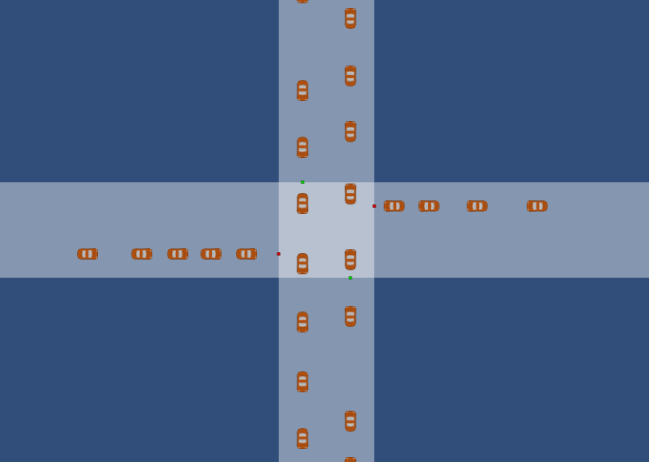
\includegraphics[height=90px]{img/intersection_tl}
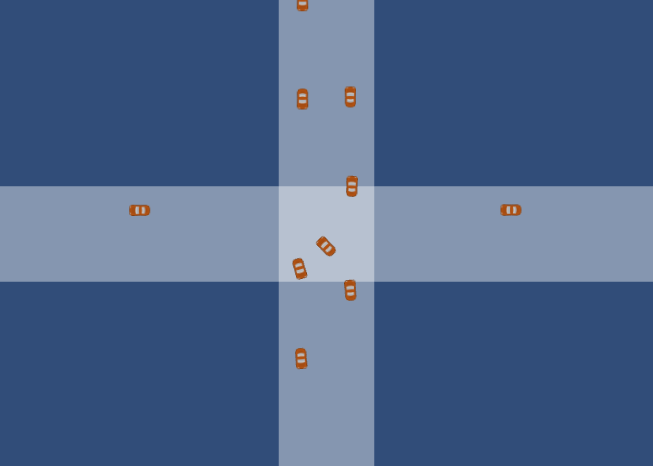
\includegraphics[height=90px]{img/intersection}
\caption{The simulation environment, with and without traffic lights}
\label{fig:intersection}
\end{figure}

\subsection{Problem Statement}
The previously obtained insights about robot control, intersection management and previous research led us to the following plan of attack:
\begin{quotation}
The goal is to explore the possibility of building a decentralized system which can guide autonomous cars through intersections. 
The current research and solutions we have found are focused around centralized systems. 

Centralized systems rely a lot on scheduling and coordination in a 'global' scale, 
while the decentralized system we envision would be built on a reactive approach which is centered around local state. 

We would like to build a prototype using the decentralized approach and compare results to an existing centralized solution.
\end{quotation}